\begin{alist}
\item Το σημείο $\text{M}\left(x, \frac{1}{2}\right)$ είναι σημείο τομής της τελικής πλευράς της γωνίας $\omega$ με τον τριγωνομετρικό κύκλο, άρα η τετμημένη του ισούται με το $\sigma\upsilon\nu\omega$ και η τεταγμένη του με το $\eta\mu\omega$. Οπότε $x = \sigma\upsilon\nu\omega$ και $\eta\mu\omega = \frac{1}{2}$

\begin{center}
\begin{tikzpicture}
\begin{axis}[
    axis lines=middle,
    xmin=-1.6, xmax=1.2,
    ymin=-1.0, ymax=1.2,
    xtick={-1.6,-1.4,-1.2,-1,-0.8,-0.6,-0.4,-0.2,0,0.2,0.4,0.6,0.8,1},
    ytick={-0.8,-0.6,-0.4,-0.2,0,0.2,0.4,0.6,0.8,1},
    grid=both,
    grid style={line width=.1pt, draw=gray!30},
    major grid style={line width=.2pt,draw=gray!50},
    thick,
    width=10cm, height=9cm,
    samples=100
]
\draw[thick] (axis cs:0,0) circle [radius=1];
\draw[thick, ->] (axis cs:0,0) -- (axis cs:-1.732, 1) node[pos=0.6, above right] {$x$};
\fill[black] (axis cs:-0.866, 0.5) circle (2pt) node[left] {$M\left(x, \dfrac{1}{2}\right)$};
\draw[dashed, thick] (axis cs:-0.866, 0) -- (axis cs:-0.866, 0.5) -- (axis cs:0, 0.5);
\fill[black] (axis cs:1, 0) circle (2pt) node[above right] {A};

\draw[fill=gray!50] (axis cs:0,0) -- (axis cs:0.2,0) arc (0:150:0.2) -- cycle;
\node at (axis cs:0.15, 0.15) {$\omega$};

\node[below right] at (axis cs:0,0) {O};
\end{axis}
\end{tikzpicture}
\end{center}

\item Γνωρίζουμε ότι $\eta\mu^2\omega + \sigma\upsilon\nu^2\omega = 1$ και από το $\alpha)$ ερώτημα $\eta\mu\omega = \frac{1}{2}$. Οπότε έχουμε ισοδύναμα:
\begin{align*}
\eta\mu^2\omega + \sigma\upsilon\nu^2\omega &= 1 \Leftrightarrow \\
\left(\frac{1}{2}\right)^2 + \sigma\upsilon\nu^2\omega &= 1 \Leftrightarrow \\
\sigma\upsilon\nu^2\omega &= \frac{3}{4} \Leftrightarrow \\
\sigma\upsilon\nu\omega &= \pm\sqrt{\frac{3}{4}} = \pm\frac{\sqrt{3}}{2}.
\end{align*}
Από το $\alpha)$ ερώτημα η τετμημένη $x$ του σημείου $\text{M}$ ισούται με το $\sigma\upsilon\nu\omega$ και $x < 0$. Άρα και $\sigma\upsilon\nu\omega < 0$, οπότε $\sigma\upsilon\nu\omega = -\frac{\sqrt{3}}{2}$.
\end{alist}
